\begin{figure*}
  \centering
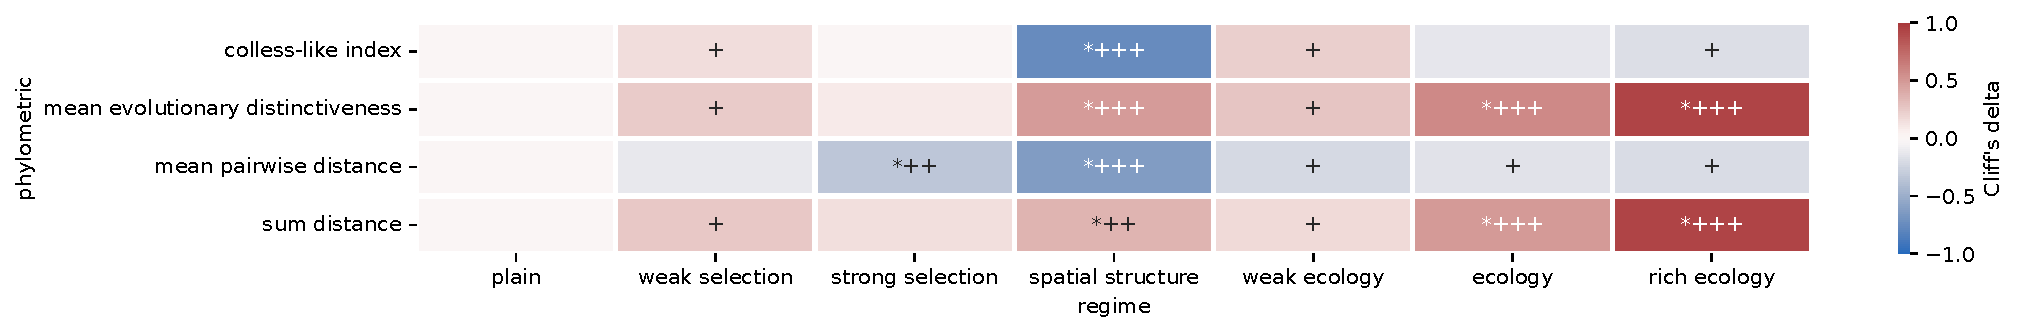
\includegraphics[width=\textwidth]{binder/binder/avida/teeplots/epoch=0+mut_distn=default+viz=heatmap+x=regime+y=phylometric+ext=.pdf}
\caption{%
  \textbf{Phylometrics for genotype-level phylogenies in Avida.}
  Tree phylometrics across surveyed evolutionary regimes, calculated on perfect-fidelity simulation phylogenies in which the taxonomic unit is genotype rather than individual.
  Note that nonparametric effect size normalization caps out to 1.0/-1.0 past the point of complete disbributional nonoverlap.
  For heatmap charts, +'s indicate small, medium, and large effect sizes using the Cliff's delta statistic and *'s indicate statistical significance at $\alpha = 0.05$ via Mann-Whitney U test.
}
  \label{fig:perfect-tree-phylometrics-heatmap-avida-genome}
\end{figure*}
